\abk{GuV}{Gewinn- und Verlustrechnung} 
\abk{AO}{Abgabenordnung} 
\abk{HGB}{Handelsgesetzbuch}
\section{Grundlagen Rechnungswesen}

\subsection{Externes Rechnungswesen}
\label{ssec:externesRechnungswesen}
\abk{Financial Accounting}{externes Rechnungswesen, Finanzwesen -- FI}
Rechnungswesen dient allgemein der Dokumentation von Leistungsaustauschbeziehungen eines Unternehmens in deren wirtschaftlichen Umfeld. Produzierte Waren oder Dienstleistungen und finanzielle Mittel stehen im Austausch und werden mittels betrieblichen Rechnungswesens vollständig erfasst, um eine unternehmerische Handlungsfähigkeit wie Planung und Steuerung zu ermöglichen. Das externe Rechnungswesen ist Bestandteil des betrieblichen Rechnungswesens und wird insbesondere zur Rechenschaftslegung und Information gegenüber externen Berichtsempfängern verwendet, um die Sicht auf die Wirtschaftlichkeit eines Unternehmens abzubilden. Externe Adressaten sind beispielsweise Gläubiger und Anteilseigner und Finanzbehörden. Für Finanzbehörden sind beispielsweise steuerrechtliche Aspekte wie z.B. Umsatz/- Gewinnsteuer relevant. Alle Stakeholder erwarten die Aussagefähigkeit einer Unternehmung hinsichtlich der Höhe des Vermögens, der Schulden, Gewinn und Verluste. 

Die Rechtsgrundlage des externen Rechnungswesens ist im Handelsrecht im  HGB (Handelsgesetzbuch) verankert. Für Unternehmen besteht eine handelsrechtliche \\Buchführungspflicht um Informationsanforderungen von Behörden erfüllen zu können, ebenso wird durch die Buchführungspflicht die nötige Transparenz für kaufmännisches Handeln im Unternehmen selbst geschaffen.

Wesentlicher Bestandteil der Buchführung ist die Finanzbuchhaltung aus dieser der Jahresabschluss (Unternehmensbilanz,  Gewinn und Verlustrechnung) erstellt wird. Externes Rechnungswesen wird auch mit der Finanzbuchhaltung und Jahresabschluss gleichgesetzt. Die Bilanz informiert über den Stand von Vermögen und Schulden eines Unternehmens. Die Finanzbuchhaltung dokumentiert
und erfasst alle Geschäftsfälle (Geld- und Güterströme) eines Geschäftsjahres.
Die Tabelle \ref{tbl2} auf Seite \pageref{tbl2} fasst die wichtigsten Merkmale des Rechnungswesens zusammen und stellt externes und internes Rechnungswesen gegenüber.

\subsubsection{Grundsätze ordnungsmäßiger Buchführung und Bilanzierung}
Die die GoB (Grundsätze ordnungsgemäßer Buchführung und Bilanzierung) beschreiben Regeln wie die Umsetzung der Buchführung im Unternehmen durchgeführt werden soll. Zu dem basieren diese Grundsätze auf ein in der Praxis angewandtes kaufmännisches Verhalten um Korrektheit der Informationen zu gewährleisten. Im HBG und AO (Abgabenordnung) finden sich wesentliche Grundsätze zur ordnungsgemäßer Buchführung und Bilanzierung wieder, allerdings sind diese Grundsätze nicht allumfassend in der Gesetzgebung (geschrieben) verankert, sondern basieren zum Teil auch auf ungeschriebene kaufmännischen Gepflogenheiten. Die GoB besagen, dass die Buchführung eines Unternehmens den Grundsätzen des Handelsrechts Folge leisten muss und das eine Buchführung nach dem formal und inhaltlich in Ordnung sein muss. 
Definition nach §238 Abs. 1 HGB besagt, dass die Buchführung \begin{quote}[...] einem sachverständigen Dritten innerhalb angemessener Zeit einen Überblick über Geschäftsvorfälle und über die Lage des Unternehmens vermitteln kann.\end{quote}

Formelle Grundsatz: Klarheit und Übersichtlichkeit
\begin{compactitem} 
\item  nach geplanten Kontenplan
\item  in einer lebenden Sprache (keine Abkürzungen)
\item  nach Belegprinzip (jede Buchung braucht einen Beleg)
\item  Offenlegung nachträglicher Veränderungen
\item  Grundsatz der Einzelerfassung und Nachprüfbarkeit
\item  zeitnahe Verbuchung der Positionen
\item  Einhaltung gesetzlicher Aufbewahrungspflichten
\end{compactitem}

Materielle Grundsatz: Vollständigkeit und Richtigkeit
\begin{compactitem}
\item  lückenlose Erfassung aller Geschäftsvorfälle
\item  Verbuchung aller Geschäftsvorfälle
\item  keine gefälschte Buchungen erzeugen
\item  Verbuchung alle Geschäftsvorfälle auf den jeweils zutreffenden Konten
\end{compactitem}
Neben den Grundsätzen der Buchführung existieren weitere Grundsätze für den Bereich der Bilanzierung. Diese haben zum Ziel, eine Bilanzwahrheit einzuhalten, welche nach den Prinzipien der Richtigkeit und Willkürfreiheit zu erfüllen ist. 

 
%Hinsichtlich der Vollständigkeit der Grundsätze der Bilanzierung, ist der Ansatzgrundsatz und Bewertungsgrundsätze zu erwähnen, welche eine weitere Detaillierungsgrad der Grundsätze ordnungsgemäßer Bilanzierung abbilden.

\subsubsection{Gewinn- und Verlustrechnung}
Die GuV (Gewinn- und Verlustrechnung) ist zusätzlich zu der Unternehmensbilanz ein Bestandteil der externen Rechungswesen eines Unternehmens. Die GuV bezieht sich auf den finanziellen Erfolg und ist im wesentlichen eine Gegenüberstellung von Aufwendungen und Erträgen, die gemäß § 242 HBG am Ende eines Geschäftsjahres zu erbringen ist. 

Die GuV bemisst alle erfolgsrelevanten Informationen, die in einer Rechungsperiode anfallen. Daher ist die periodengerechte Erfassung aller Geschäftsvorfälle (z.B. Inventur) von Bedeutung. Die Buchungen von Aufwänden und Erträgen in Erfolgskonten und deren Saldierung und Abschluss im GuV-Konto, fließen als Ergebnis über das Eigenkapital-Konto letztlich in die Schlussbilanzen der Unternehmen ein.

\abk{GoB}{Grundsätze ordnungsgemäßer Buchführung und Bilanzierung}
\subsubsection{Jahresabschluss nach HGB und IFRS}

\subsection{Internes Rechnungswesen}
\label{ssec:internesRechnungswesen}
\abk{Management Accounting}{internes Rechnungswesen, Controlling -- CO}

Der Bereich des betrieblichen Rechnungswesens übernimmt eine besondere Dokumentations- und Kontrollfunktion in einer Wirtschaftsunternehmung.
Die externen orientierten Aufgaben sind meist durch gesetzliche Vorgaben eingeschränkt und dienen der Rechenschaftslegung gegenüber Gesellschaftern, Gläubigern, der Öffentlichkeit und dem Staat (Vgl. s. Kapitel \ref{ssec:externesRechnungswesen} auf S. \pageref{ssec:externesRechnungswesen}).
Die intern orientierten Aufgaben unterliegen hingegen keinerlei sachfremden und gesetzlichen Vorgaben und können so den individuellen Ansprüchen des Managements angepasst werden. Das interne Rechnungswesen (Betriebsbuchhaltung oder Management Accounting) dient der mengen- und wertmäßig Erfassung sowie\\ Überwachung aller in einem Unternehmen auftretenden Geld- und Leistungsströme. Es ist typischerweise kurzfristig ausgerichtet und weist kürzere Abrechnungszeiträume als das Geschäftsjahr des externen Rechnungswesens auf\footnote{Vgl. \cite{Wohe2000}, S. 853}\footnote{Vgl. \cite{Schierenbeck2008}, S. 799}.
Die Tabelle \ref{abb1} (S. \pageref{abb1}) stellt die wichtigsten Unterscheidungsmerkmale zwischen dem internen und dem externen Rechnungswesen dar.\\
\begin{table}[htbp]
\begin{center}
\caption[Vergleich externes- und internes Rechnungswesen]{Vergleich externes- und internes Rechnungswesen}
\includegraphics[width=1\textwidth]{Images/VergleichIntExt.png}
\label{abb1}
{\footnotesize In Anlehnung an: \cite{Lojewski2001}, S. 6}
\end{center}
\end{table} 
\noindent Es ergeben sich 3 Hauptaufgaben im internen Rechnungswesen\footnote{Vgl. ebd., S. 799}:
\begin{compactitem}
\item[1] Die Ermittlung des kurzfristigen Betriebserfolgs
\item[2] Kontrolle der Wirtschaftlichkeit und Budgetierung
\item[3] Rechnerische Fundierung unternehmenspolitischer Entscheidungen
\end{compactitem}

\subsubsection{Ermittlung des kurzfristigen Betriebserfolgs}
Zur Erfüllung der genannten Hauptaufgaben der internen Unternehmungsrechnung kommen die Systeme der Kosten- und Leistungsrechnung zum Einsatz\footnote{Vgl. \cite{Schierenbeck2008}, S.~800}. Nach Jörg Wöltje besteht das interne Rechnungswesen aus der Kostenrechnung, der Leistungsrechnung und der Erfolgsrechnung. Die Kostenrechnung dokumentiert die Verbrauchsseite, also die entstandenen Kosten des Produktionsprozesses. Die Leistungsrechnung dokumentiert die Entstehungsseite, also die erzielten Erlöse des Produktionsprozesses. Stellt man Verbrauchs- und Entstehungsseite gegenüber, spricht man von einer Erfolgsrechnung. Die kalkulatorische Erfolgsrechnung als Hauptbestandteil des internen Rechnungswesens wird für einzelne Produkte, Produktgruppen oder Unternehmensbereiche erstellt und soll für kurze Abrechnungszeiträume den Betriebserfolg als Saldo der bewerteten Periodenleistungen und der Periodenkosten ermitteln\footnote{Vgl. \cite{Woltje2008}, S.~179}.
Kernstück ist dabei die Kostenrechnung, die bei entsprechender Ausgestaltung den Prozess der Kostenentstehung schrittweise verfolgt und eine rechnerische Aufgliederung des Kostengefüges 
\begin{compactitem}
\item nach Kostenarten (Welche Kosten fallen an?), 
\item nach Kostenstellen (Wo fallen welche Kosten an?) und 
\item nach Kostenträgern (Wofür, d.h. für welche Leistungen fallen Kosten an?)
\end{compactitem} ermöglicht\footnote{Vgl. \cite{Schierenbeck2008}, S.~799}\footnote{Vgl. \cite{Ossadnik2008}, S~52 ff.}.


\subsubsection{Kontrolle der Wirtschaftlichkeit und Budgetierung}
Wie wirtschaftlich wird in den Kostenstellen gearbeitet?
Aufgrund ihrer internen Ausrichtung fällt der kalkulatorischen Erfolgsrechnung die Aufgabe zu, den Ablauf der Unternehmungsprozesse zu überwachen. Klein sieht in der Kontrolle die Überwachung von Dispositionen untergeordneter Instanzen. Dabei kann Kontrolle definiert werden als die \glqq Durchführung eines Vergleichs zwischen einer zu prüfenden und einer Plangröße\grqq \footnote{Vgl. \cite{Klein1999}, S.~22}.
Dieses Instrument zeigt, welche Produkte am stärksten am Umsatz beteiligt sind. Auch wird klar, welche Produktelemente die höchsten Kosten verursachen und deshalb besonders beachtet werden sollten. So werden Schwachstellen und Unwirtschaftlichkeiten im Leistungserstellungsprozesses erkannt\footnote{Vgl. \cite{Woltje2008}, S.~196 f.}. Mit dem Ziel, vorgegebene Kostendeckungs-, Gewinn- oder Rentabilitätsziele sicher zu stellen, wird die kalkulatorische Erfolgsrechnung auch für die Budgetierung von Kosten und Erlösen eingesetzt\footnote{Vgl. \cite{Schierenbeck2008}, S.~800}.

\subsubsection{Rechnerische Fundierung unternehmenspolitischer Entscheidungen}
Der internen Unternehmungsrechnung kommt hier die Aufgabe zu, das Zahlenmaterial für Entscheidungsrechnungen im Sinne von Planungsrechnungen zu liefern. Diese Funktion dient sowohl der Entscheidungsfindung als auch dem Entscheidungsvollzug\footnote{Vgl. \cite{Klein1999}, S.~22}\footnote{Vgl. \cite{Schierenbeck2008}, S.~800}.\\
Zu den Hauptaufgaben zählen hier in erster Linie\footnote{Vgl. ebd., S.~800}: 
\begin{compactitem}
\item die Kalkulation von Preisen und Preisuntergrenzen, 
\item die Planung des Mitteleinsatzes im Marketing, 
\item die Produktions- und Absatzplanung, 
\item die Produktionsdurchführungsplanung, 
\item die Materialbereitstellungsplanung (einschließlich Wahl zwischen Eigenfertigung und Fremdbezug) \\sowie 
\item die Investitions- und Finanzierungsprogrammplanung. 
\end{compactitem} 





%Das Projektcontrolling ist neben der Projektplanung und Führung eine Instanz des Projektmanagements. Auch in anderen Betriebswirtschaftlichen Bereichen ist das Controlling etabliert. In diesem Kapitel wird anhand der allgemeinen Definitionen, der Brückenschlag zwischen Controlling und dem Projektcontrolling aufgezeigt.
%\subsection{Projekt und Projektmanagement}
%\label{ssec:Projekt}
%Um gleich zu Beginn ein einheitliches Verständnis zu schaffen, bedarf es der grundsätzlichen Definition der Begriffe Projekt und Projektmanagement.
%
%Projekte sind heute nicht mehr wegzudenken und in allen Bereichen der Wirtschaft in unterschiedlichsten Ausprägungen zu finden. Gerade neuartige, einmalige oder besonders komplexe Vorhaben lassen sich nicht in bestehenden Linienorganisationen bearbeiten und erfordern meist interdisziplinäre Organisationen. \label{69901Projekt} Die DIN 69901 definiert ein Projekt als ein Vorhaben, das im Wesentlichen gekennzeichnet ist durch:
%\begin{compactitem}
%\item die Einmaligkeit der Bedingungen 
%\item eine projektbezogene Zielvorgabe 
%\item eine zeitliche, finanzielle und personelle Begrenzung 
%\item Abgrenzung gegenüber anderen Projekten 
%\item eine projektspezifische Organisation
%\end{compactitem}
%%\begin{figure}[htbp]
%\begin{floatingfigure}[r]{0.4\textwidth} 
%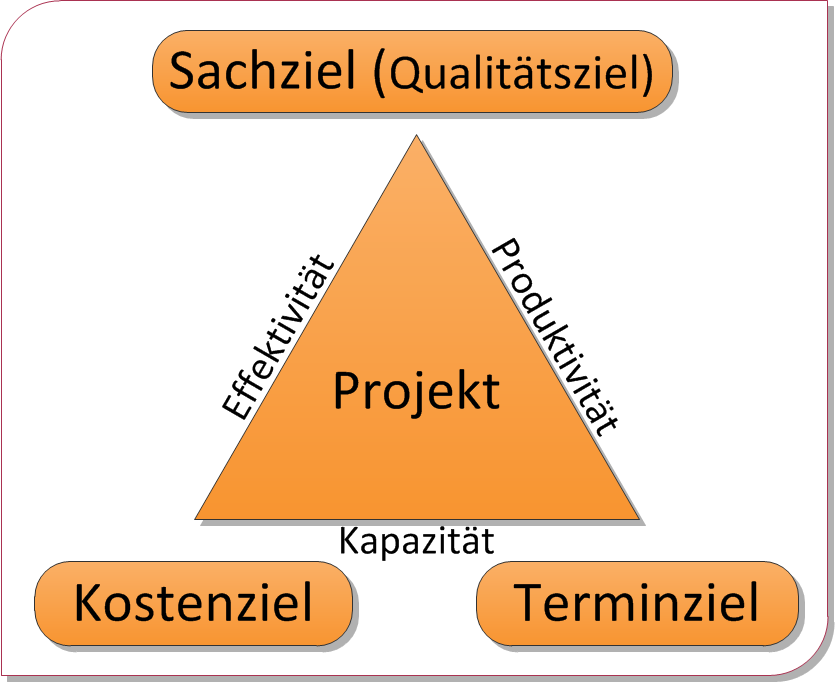
\includegraphics[width=0.4\textwidth]{Images/magischesDreieck.png}
%\begin{center}
%   {\footnotesize In Anlehnung an: \cite{Wischnewski1991}}
%   \caption[Magisches Dreieck]{Magisches Dreieck}\label{abb2}
%\end{center}
%\end{floatingfigure}\noindent
%Es stellt sich die Frage, welche Parameter entscheidend für den Erfolg eines Projektes sind. Aus den oben genannten Merkmalen lassen sich die Parameter Qualität des Ergebnisses (Sachziel), Kosten (Kostenziel) und Dauer (Terminziel) ableiten. Diese Ziele beeinflussen sich gegenseitig und bilden das so genannte „magische“ Dreieck der Projektorganisation (siehe Abbildung \ref{abb2} auf S. \pageref{abb2})\footnote{Vgl. \cite{Wegmann&Winklbauer2006}}
%Typisch für viele Projekte ist, dass man anfangs nicht weiß, ob die angestrebten Ziele überhaupt erreicht werden können. Häufig wird der Zeitrahmen nicht eingehalten, die Kosten werden überschritten, oder man ist nicht in der Lage, die erhoffte Qualität zu erbringen\footnote{Vgl. \cite{Fiedler2008}, S.~3}.
%
%Die Aufgabe des Projektmanagements besteht darin, dafür zu sorgen, dass das Vorhaben unter der Berücksichtigung der Projektziele durchgeführt wird. Das Projektmanagement nimmt dabei bestimmte Funktionen wie etwa Planung, Führung und Controlling wahr\footnote{Vgl. \cite{Bergmann&Garrecht2008}, S.~209}. Nach DIN 69901 versteht man unter dem Begriff  Projektmanagement: \label{69901Projektmgmt}\begin{quote}Projektmanagement ist die Gesamtheit von Führungsaufgaben, -organisation, -techniken und –mitteln für die Abwicklung eines Projekts.\end{quote}\par 
%
%\subsection{Controlling}
%\label{ssec:c}
%Controlling hat sich in den letzten Jahren zu einer festen Institution in den Unternehmen entwickelt. Es gibt kaum ein Unternehmen, das keine eigene Abteilung oder zumindest Angestellte hat, die für das Controlling verantwortlich ist. Der Begriff Controlling ist allerdings sehr weit gefasst. Die Anforderungen in den Unternehmen sind so komplex, dass sich das Controlling dezentralisieren muss, um seine Aufgabe erfüllen zu können. Der Controller kann als ein \glqq Beifahrer\grqq  definiert werden, der den \glqq Fahrer\grqq (Manager) beim Steuern des \glqq Fahrzeugs\grqq \ (Unternehmen) unterstützt. Der Fahrer konzentriert sich auf das Steuern und auf die möglichen Reaktionen. Diese Aktivitäten verlangen seine volle Aufmerksamkeit und er kann keine anderen Tätigkeiten wie etwa Kartenlesen verrichten. Der Beifahrer ist freier als der Fahrer. Er kann daher nützliche Dinge tun, die den Fahrer unterstützen\footnote{Vgl. \cite{Pufahl2006}, S.~11}.\newpage
%\begin{floatingfigure}[r]{0.37\textwidth} 
%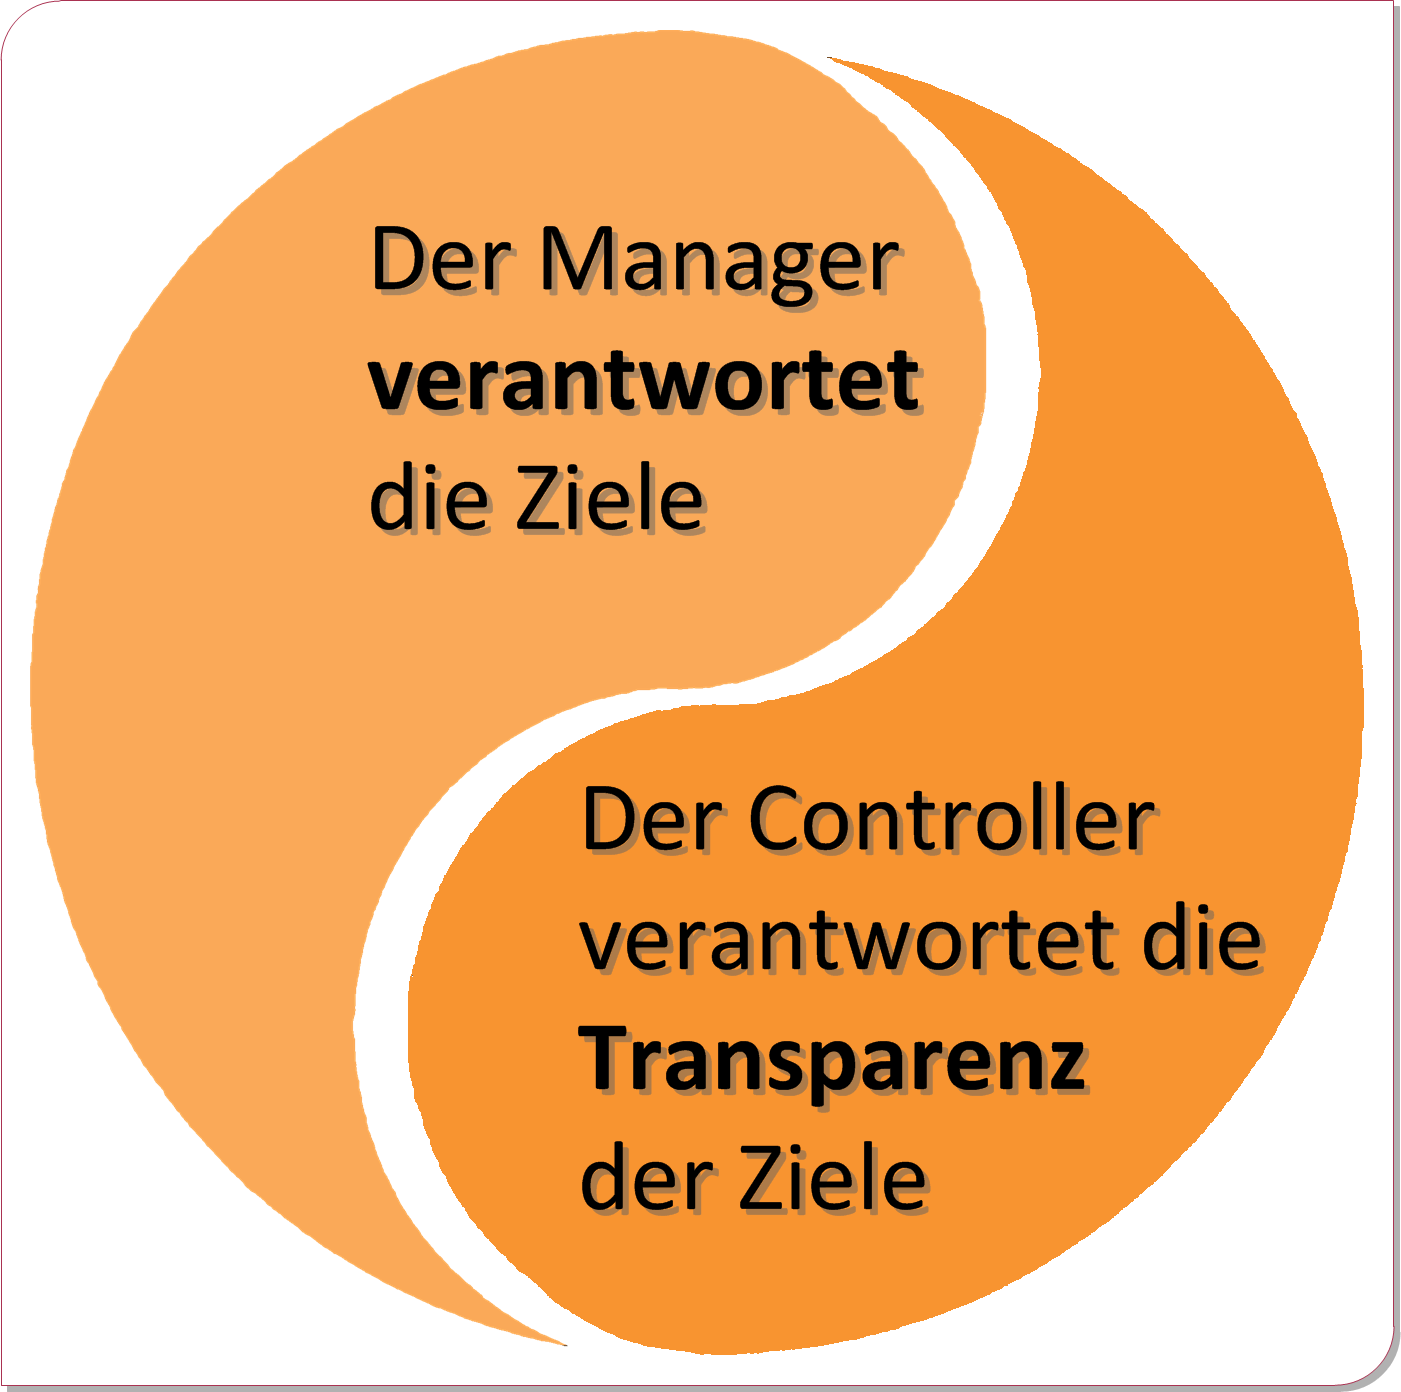
\includegraphics[width=0.37\textwidth]{Images/aufgabenabgrenzungLeiterController.png}
%\begin{center}
%   {\footnotesize In Anlehnung an: \cite{Fiedler2008}, S. 21}
%   \caption[Management vs. Controlling]{Management vs. Controlling}\label{abb4}
%\end{center}
%
%%\end{figure}
%\end{floatingfigure}\noindent
%Controlling hat primär die Aufgabe, zwischen Planung, Kontrolle und Informationsversorgung zu koordinieren (so genannte systemkoppelnde Funktion des Controllings). Die Daten der Planung sind beispielsweise so aufzubereiten, dass eine Kontrolle möglich wird.  Auch innerhalb der Planung und Kontrolle sind Abstimmungen erforderlich. Es muss z. B. der Absatzplan mit dem Produktionsplan und dieser wiederum mit dem Investitionsplan koordiniert werden. Das Controlling stellt auch die Abbildung der strategischen Ziele in der operativen Perspektive sicher. Wichtig ist auch die Gestaltung der genannten Aufgabenbereiche, also die Schaffung von Strukturen und Prozessen. Die systembildende Funktion des Controllings regelt beispielsweise, welche Pläne zu erstellen sind und wie deren Kontrolle funktioniert. Hierzu werden die geeigneten Instrumente und Methoden, sowie die Verantwortlichen festgelegt\footnote{Vgl. \cite{Fiedler2008}, S.~10 f.}.
%\subsection{Projektcontrolling}
%\label{ssec:pc}
%Die DIN 69901 beschreibt das Projektcontrolling als Regelkreis:\begin{quote}Sicherung des Erreichens der Projektziele durch: Soll-Ist-Vergleich, Feststellung der Abweichungen, Bewerten der Konsequenzen und Vorschlagen von Korrekturmaßnahmen, Mitwirkung bei der Maßnahmenplanung und Kontrolle der Durchführung.
%\end{quote}
%Für das Verständnis ist es wichtig, die Stellung des Projektcontrollings zum allgemeinen Unternehmenscontrolling und zum Projektmanagement herauszuarbeiten (Vgl. Abbildung \ref{abb3} auf Seite \pageref{abb3}). Die Begriffe Einzelprojektcontrolling, Multiprojektcontrolling und strategisches Projektcontrolling werden nicht einheitlich verwendet. Üblich ist es auch, das strategische Projektcontrolling als strategisches Multiprojektcontrolling oder Portfoliocontrolling zu bezeichnen.
%\begin{figure}[htbp]
%%\begin{floatingfigure}[r]{0.7\textwidth} 
%\includegraphics[width=1\textwidth]{Images/stellungProjektcontrolling.png} 
%\begin{center}
%   {\footnotesize In Anlehnung an: \cite{Fiedler2008}, S. 13 u. 23}
%   \caption[Stellung des Projektcontrollings]{Stellung des Projektcontrollings}\label{abb3}
%\end{center}
%\end{figure}
%%\end{floatingfigure}
%Die Abbildung \ref{abb3} auf Seite \pageref{abb3} zeigt, dass sich das Projektcontrolling als Bindeglied zwischen dem Unternehmenscontrolling und dem Projektmanagement wiederfindet.
%Die Strategien, Ziele und Werte des Unternehmens werden so in die Gestaltung der Prozesse und Strukturen einfließen. Anders herum sind die Daten des Projektes für den Erfolg und die Liquidität des Unternehmens relevant. [...]tbd
%Das Projektmanagement wird bei der Wahrnehmung der Führungsaufgaben und Koordination unterstützt\footnote{Vgl. \cite{Fiedler2008}, S.~13 f.}.
%
%Zu unterscheiden sind Einzelprojektcontrolling, Multiprojektcontrolling und strategisches Projektcontrolling. Neben den unterschiedlichen strategischen bzw. operativen Ausrichtungen, sind diesen Bereichen auch unterschiedliche Aufgabenschwerpunkte zuzuordnen.
%Ziel des Einzelprojektcontrollings ist es, das Projektmanagement so zu unterstützen, dass ein einzelnes Projekt bezüglich der Projektziele Qualität, Kosten und Zeit erfolgreich abgewickelt wird. Einzelprojektcontrolling orientiert sich an den Lebenszyklusphasen des Projektes und stellt dem Projektmanagement sowohl phasenspezifische wie auch phasenübergreifende Instrumente zur Verfügung.
%
%Beim Multiprojektcontrolling werden mehrere Projekte mit unterschiedlichen Terminen und Fertigstellungsständen für eine Abrechnungsperiode zusammengefasst betrachtet. Ziel ist es, die Projektprogramm- und Projektablaufplanung unter Beachtung
%\begin{compactitem}
%\item der Kapazitätsgegebenheiten,
%\item der Kosten- und Finanzwirkungen sowie
%\item möglicher weiterer Nebenbedingungen(z. B. strategische Ziele des Unternehmens)
%\end{compactitem}
%zu einem gemäß den Bereichs- bzw. Unternehmenszielen bestmöglichen Gesamtgefüge zu koordinieren. Die Instrumente des Multiprojektcontrollings sind im Prinzip die gleichen wie beim Einzelprojektcontrolling, nur mit dem Unterschied, dass mehrere Projekte gleichzeitig bzw. zu einer Gruppe verdichtet betrachtet werden. Diese operativen Projektaspekte werden im Kapitel \ref{sec:opc} auf Seite \pageref{sec:opc} ausführlich behandelt.
%
%Die Form des strategischen Projektcontrollings befasst sich mit strategischen Aufgabenstellungen des Projektmanagements. Dazu gehört die Bereitstellung von Informationen und Instrumenten zur effektiven Projektbewertung und Projektauswahl\footnote{Vgl. \cite{Fiedler2008}, S.~14--16}. Das strategische Projektkontrolling wird im nachfolgenden Kapitel \ref{sec:spc} detailliert beschrieben.
%
%
